\documentclass[10pt]{article}

% --- Small page margins (small border distance) ---
\usepackage[a4paper,margin=1.2cm]{geometry}

\usepackage[utf8]{inputenc}
\usepackage[T1]{fontenc}
\usepackage{amsmath,amssymb}
\usepackage{graphicx}
\usepackage{subcaption}
\usepackage{booktabs}
\usepackage[hidelinks]{hyperref}
\usepackage{titlesec}

\graphicspath{{../graphs/}}

% Tighter spacing to keep the border distance visually small
\setlength{\parskip}{1pt}
\setlength{\parindent}{0pt}

% Compact captions and display-math spacing
\usepackage{caption}
\captionsetup{font=small,skip=2pt}
\setlength{\abovedisplayskip}{3pt}
\setlength{\belowdisplayskip}{3pt}
\setlength{\abovedisplayshortskip}{2pt}
\setlength{\belowdisplayshortskip}{2pt}

% --- Smaller headings + tighter space between headings and text ---
% \titlespacing*{<cmd>}{left}{before-space}{after-space}
\titleformat{\section}{\normalfont\large\bfseries}{\thesection}{0.6em}{}
\titlespacing*{\section}{0pt}{4pt}{1pt}
\titleformat{\subsection}{\normalfont\normalsize\bfseries}{\thesubsection}{0.6em}{}
\titlespacing*{\subsection}{0pt}{3pt}{1pt}
\titleformat{\subsubsection}{\normalfont\small\bfseries}{\thesubsubsection}{0.6em}{}
\titlespacing*{\subsubsection}{0pt}{2pt}{0pt}

\begin{document}

% --- Title block matching the source PDF ---
\begin{center}
  {\large\bfseries Finite-time Analysis of the Multi-armed Bandit Problem}\\[3pt]
  {\itshape by Auer, Cesa-Bianchi \& Fischer (2002), Machine Learning 47:235--256}\\[1pt]
  {\bfseries Paper Summary -- Seminar ``Decision Making Algorithms''}\\[1pt]
  {\itshape Presented by Ali Kaya, Egemen Bulut, Korbinian Knestel}
\end{center}
\vspace{2pt}
\hrule
\vspace{4pt}

\section{Motivation and Problem}
How can an agent maximize cumulative reward when making repeated decisions under uncertainty? Its canonical
form is the \emph{multi-armed bandit}: a player faces $K$ machines (``arms'') with unknown reward distributions
and must choose one each round, trading off \emph{exploitation} (playing the best-looking arm) against
\emph{exploration} (trying others underestimated by chance). Lai and Robbins (1985) showed regret must grow at
least logarithmically in the number of plays $n$, but only \emph{asymptotically}. This paper gives efficient
policies achieving logarithmic regret \emph{uniformly over time} -- matching the finite horizon of real applications.

\section{Setup}
Each arm $i$ yields independent identically distributed rewards with unknown mean $\mu_{i}$, independent
across arms. Let $T_{i}(n)$ be the number of plays of arm $i$ in the first $n$ rounds, $\bar{X}_{i}$ its
sample mean, $\mu^{*}=\max_{i}\mu_{i}$ the best mean, and $\triangle_{i}=\mu^{*}-\mu_{i}$ the
suboptimal gap. The performance of the policies is measured with regret, the difference between the
expected reward of playing the policy and playing always the best arm:
\[
\text{Regret}=\mu^{*}n-\sum_{j=1}^{K}\mu_{j}\,\mathbb{E}[T_{j}(n)]
\]

\section{Algorithms, Guarantees and Proof Ideas}

\subsection{UCB1}
At round $n$, play the machine $j$ that maximizes $\bar{x}_{j}+\sqrt{(2\ln n)/n_{j}}$, where $\bar{x}_{j}$ is the average reward of
machine $j$ and $n_{j}$ is its number of plays so far. Initialization requires playing each of the $K$ machines once.
This mechanism allows machines with a low average reward to be played again, ensuring that a
high-performing machine that initially performed poorly due to bad luck can still be discovered.

\subsubsection{Theorem 1}
For all $K>1$, the expected cumulative regret is bounded logarithmically relative to the number of plays
$n$. This regret bound is derived using the Chernoff-Hoeffding bound. The main objective of the proof is to
bound the probability of playing a suboptimal machine that does not maximize the true mean reward.

\subsection{UCB1-Tuned}
By changing the exploration bonus of UCB1, we can create a variant called UCB1-Tuned. This version
shows better results in experiments, but a mathematical regret bound cannot be proven. The new exploration
bonus is defined as $\sqrt{(\ln n/n_{j})\min\{1/4,\,V_{j}(n_{j})\}}$, where
\[
V_{j}(s)=\left(\frac{1}{s}\sum_{\tau=1}^{s}X_{j,\tau}^{2}\right)-\bar{x}_{j}^{2}+\sqrt{(2\ln n)/s}.
\]

\subsection{UCB2}
To minimize the large constant factors of UCB1, UCB2 introduces an epoch-based structure. Instead of
playing a selected machine only once, the algorithm plays the chosen machine $j$ sequentially for a specific
block of trials, called an epoch, of length $\tau(r_{j}+1)-\tau(r_{j})$, where $\tau(r)=\lceil(1+\alpha)^{r}\rceil$ and $0<\alpha<1$. At
the end of these epochs, an arm $j$ is selected by maximizing the sum of its average reward $\bar{x}_{j}$ and the
exploration bonus term
\[
a_{n,r_{j}}=\sqrt{\frac{(1+\alpha)\ln\!\big(en/\tau(r_{j})\big)}{2\,\tau(r_{j})}}.
\]

\subsubsection{Theorem 2}
For all $\alpha>0$ and $K>1$, the expected regret is bounded logarithmically. Similar to UCB1, the proof
utilizes the Chernoff-Hoeffding bound to control suboptimal plays. However, it splits the analysis to treat
early epoch errors as a fixed penalty, which introduces a time-independent constant term $c_{\alpha}/\triangle_{i}$ into the
cumulative regret equation; a smaller $\alpha$ optimizes the long-term rate but causes this constant to increase.

\subsection{$\varepsilon_{n}$-GREEDY}
With probability $\varepsilon_{n}=\min\!\big\{1,\,cK/(d^{2}n)\big\}$ play a random arm, else the empirical best. Here $c>0$ a tuning
constant, $K$ the number of arms, $d$ a known lower bound on the gap between the best and second best arm. A
decaying $\varepsilon_{n}$ is essential since constant $\varepsilon$ gives linear regret.

\subsubsection{Theorem 3}
For $n\geq cK/d$, it bounds $P\{\text{pull suboptimal arm } j \text{ at round } n\}$ by order $c/(d^{2}n)+o(1/n)$, which integrates
out to logarithmic regret, given a known lower bound $d\leq\min_{i}\triangle_{i}$. The proof splits that probability into a
random exploration term and an exploitation term. The exploration term is already an exact quantity -- there is
nothing to bound -- so all the risk is in the exploitation term, which is bounded via Chernoff-Hoeffding and
re-expressed using only $j$'s purely random pulls, whose count is controlled directly by Bernstein's inequality.

\subsection{UCB1-Normal}
Unlike the other policies, which assume bounded rewards $[0,1]$, UCB1-Normal assumes normal rewards
with both mean and variance unknown, estimating each arm's variance from its data gathered through its
trials. For each round $n=1,2,\dots$:
\begin{itemize}\setlength{\itemsep}{0pt}\setlength{\parskip}{0pt}\setlength{\topsep}{1pt}
  \item If there is a machine played less than $\lceil 8\log n\rceil$ times play this machine.
  \item Otherwise play machine $j$ that maximizes
  \[
  \bar{x}_{j}+\sqrt{16\,\frac{q_{j}-n_{j}\bar{x}_{j}^{2}}{n_{j}-1}\cdot\frac{\ln(n-1)}{n_{j}}},
  \]
  where $q_{j}$ is the sum of squared rewards obtained from machine $j$.
  \item Update $\bar{x}_{j}$ and $q_{j}$ with obtained reward $x_{j}$.
\end{itemize}

\subsubsection{Theorem 4}
For all $K>1$, if UCB1-Normal is run on $K$ arms with normal distributions $P_{1},\dots,P_{K}$ with
means $\mu_{i}$, variances $\sigma_{i}^{2}$, its expected regret after $n$ plays is at most:
\[
256(\log n)\!\left(\sum_{i:\mu_{i}<\mu^{*}}\frac{\sigma_{i}^{2}}{\triangle_{i}}\right)+\left(1+\frac{\pi^{2}}{2}+8\log n\right)\!\left(\sum_{j=1}^{K}\triangle_{j}\right).
\]
Each suboptimal arm contributes $256\,\sigma_{i}^{2}/\triangle_{i}$, and the forced exploration
shows the regret in the $\lceil 8\log n\rceil$ term. This results in a higher logarithmic factor than the other
policies.

\section{Experiments}
Our simulations reproduce all policies across distributions of varying difficulties, comparing UCB1-Tuned,
UCB2, and $\varepsilon_{n}$-GREEDY (at several $c$ values) on Distribution 2 $[0.9, 0.8]$, Distribution 12 $[0.9, 0.8\times3,
0.7\times3, 0.6\times3]$, Distribution 13 $[0.9, 0.8\times9]$, and Distribution 14 $[0.55, 0.45\times9]$. Figure~\ref{fig:ratio} reports the share of
plays on the best arm and Figure~\ref{fig:regret} reports cumulative regret.

\begin{figure}[htb]
\centering
\begin{subfigure}[b]{0.235\textwidth}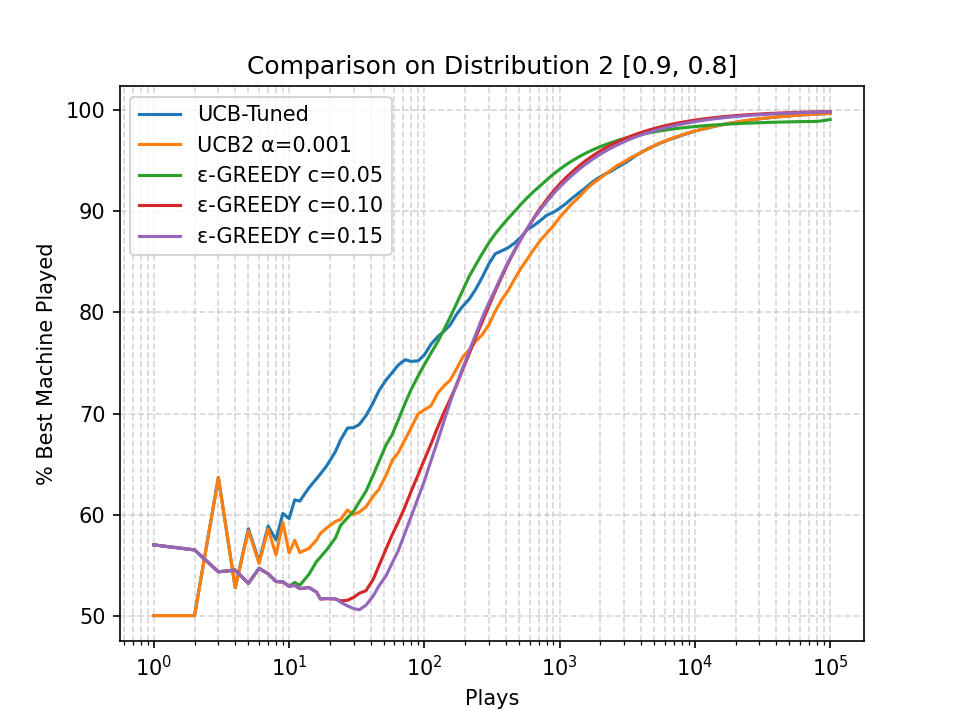
\includegraphics[width=\linewidth,height=3.1cm]{comparison_dist2_ratio.png}\end{subfigure}\hfill
\begin{subfigure}[b]{0.235\textwidth}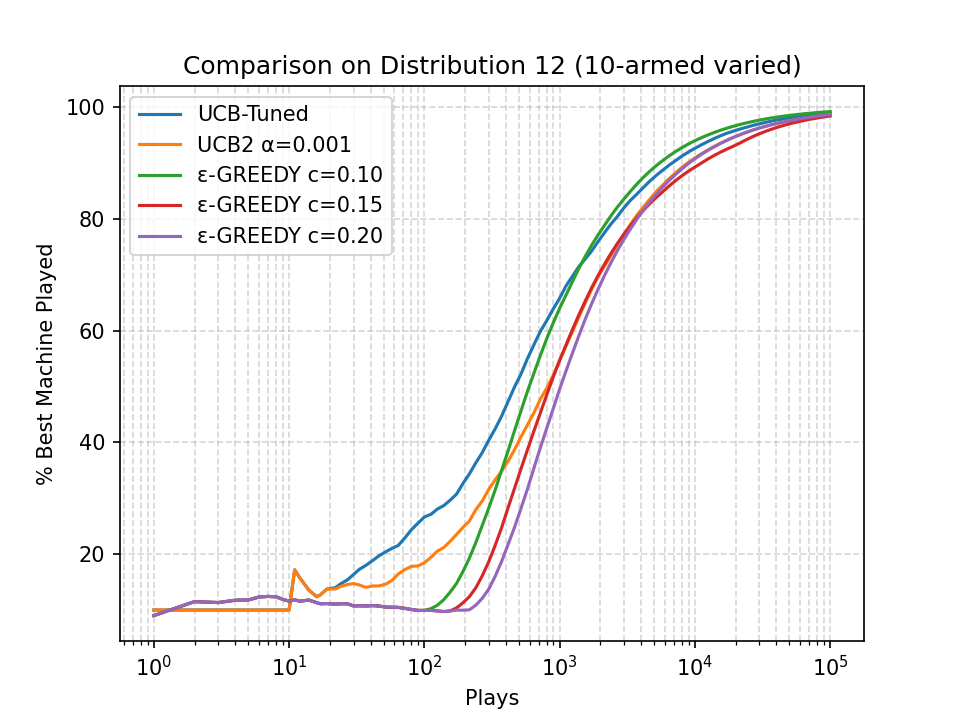
\includegraphics[width=\linewidth,height=3.1cm]{comparison_dist12_ratio.png}\end{subfigure}\hfill
\begin{subfigure}[b]{0.235\textwidth}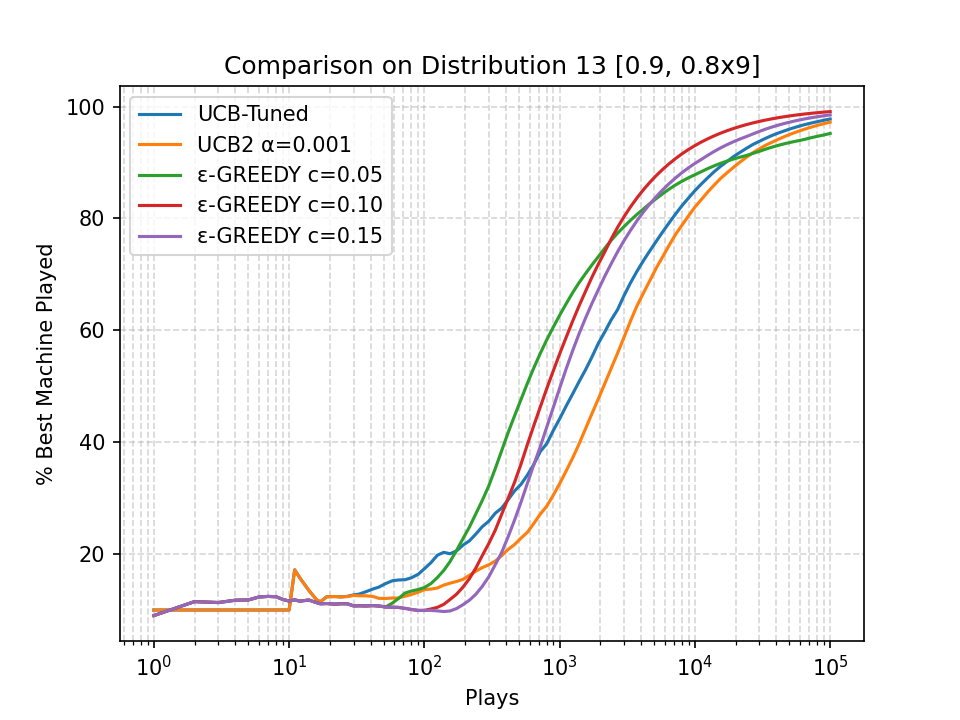
\includegraphics[width=\linewidth,height=3.1cm]{comparison_dist13_ratio.png}\end{subfigure}\hfill
\begin{subfigure}[b]{0.235\textwidth}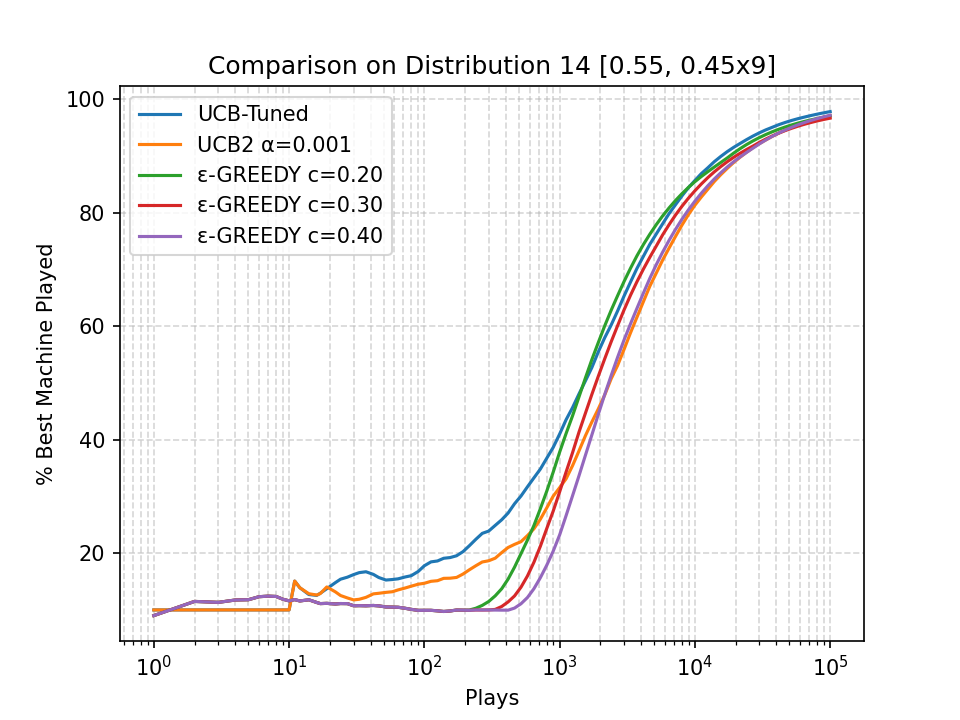
\includegraphics[width=\linewidth,height=3.1cm]{comparison_dist14_ratio.png}\end{subfigure}
\caption{Cross-algorithm comparison -- \% best machine played across the four distributions.}
\label{fig:ratio}
\end{figure}

\begin{figure}[htb]
\centering
\begin{subfigure}[b]{0.235\textwidth}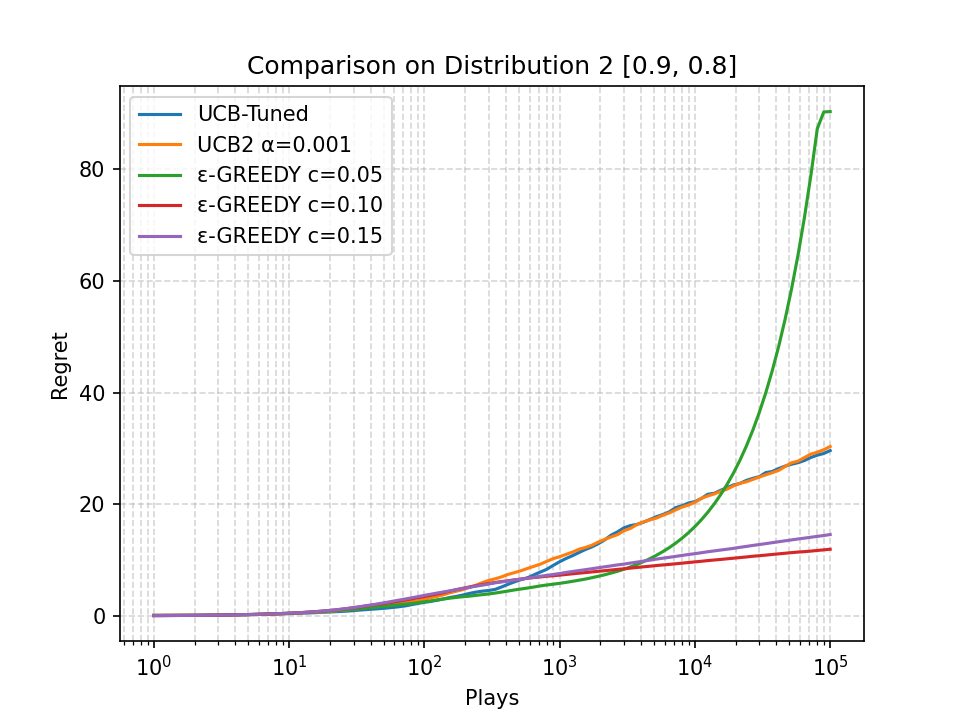
\includegraphics[width=\linewidth,height=3.1cm]{comparison_dist2_regret.png}\end{subfigure}\hfill
\begin{subfigure}[b]{0.235\textwidth}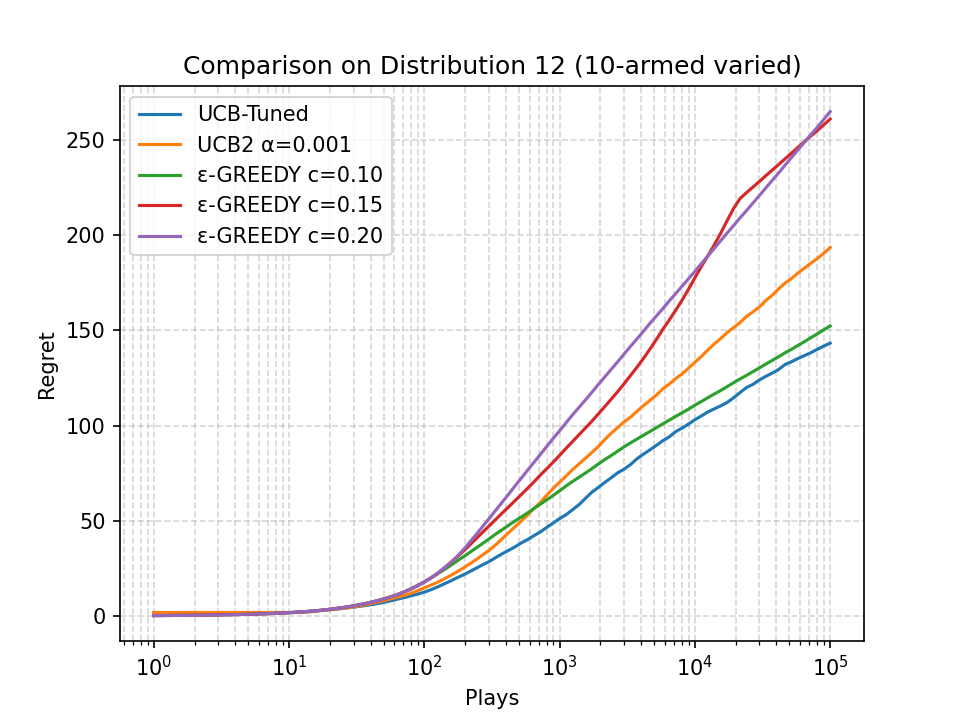
\includegraphics[width=\linewidth,height=3.1cm]{comparison_dist12_regret.png}\end{subfigure}\hfill
\begin{subfigure}[b]{0.235\textwidth}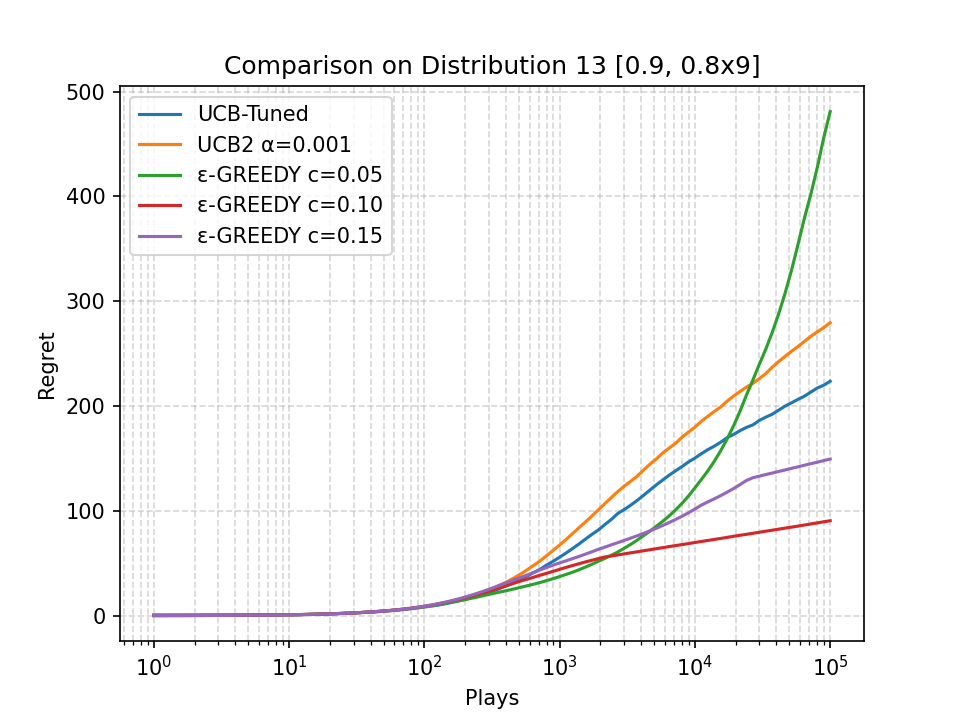
\includegraphics[width=\linewidth,height=3.1cm]{comparison_dist13_regret.png}\end{subfigure}\hfill
\begin{subfigure}[b]{0.235\textwidth}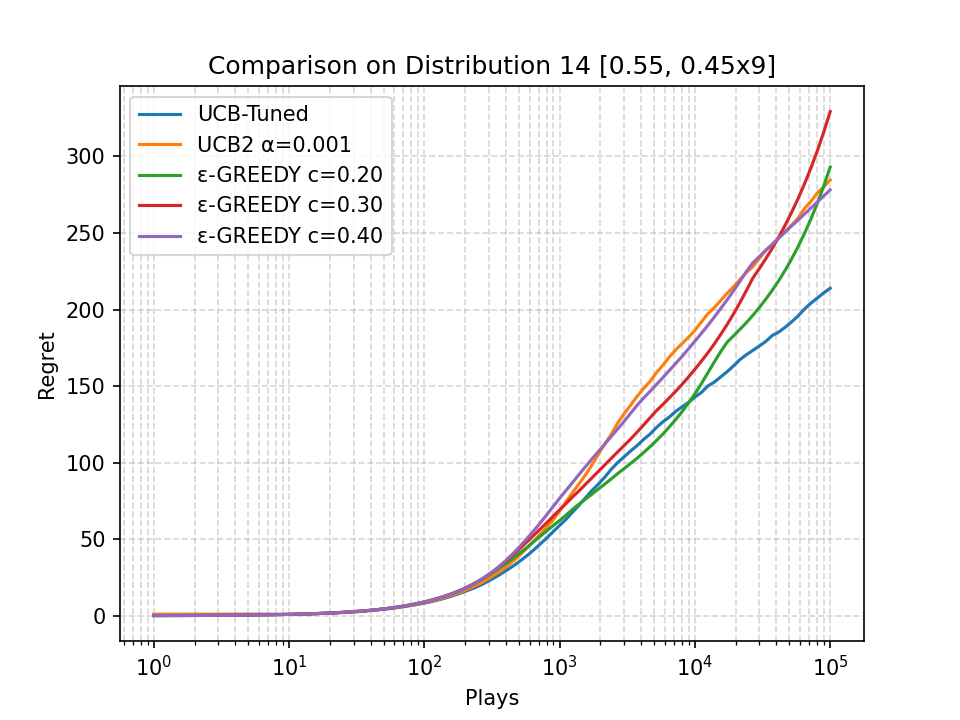
\includegraphics[width=\linewidth,height=3.1cm]{comparison_dist14_regret.png}\end{subfigure}
\caption{Cross-algorithm comparison -- cumulative regret across the four distributions.}
\label{fig:regret}
\end{figure}

On easy two-arm problems (Dist 2) a well-tuned $\varepsilon_{n}$-GREEDY ($c\approx0.10$) is the clear winner, with
UCB1-Tuned and UCB2 close behind. But $\varepsilon_{n}$-GREEDY is fragile: on Dist 12 and 14, where uniform
exploration wastes equal pulls on both terrible and competitive arms, it breaks down while UCB1-Tuned
adapts and dominates -- the paper's signature finding. Dist 13 shows the weakness is specific to widely spread
losers rather than arm count, since $\varepsilon_{n}$-GREEDY again wins there. The best $c$ spans roughly an $8\times$ range
across distributions, confirming the authors' remark that no single value works well for all problems. Overall
UCB2 tracks UCB1-Tuned but stays consistently slightly worse, while UCB1-Tuned is stable and largely
insensitive to reward variance.

\section{Strengths, Weaknesses and Takeaway}
\textbf{Strengths:} the first finite time logarithmic regret guarantees; results hold for any bounded support reward
distribution; and Theorems 1--3 remain valid under mild reward dependence. \textbf{Weaknesses:} UCB1's leading
constant is about $16\times$ the Lai-Robbins optimum; UCB1-Normal rests on unproven conjectures;
$\varepsilon_{n}$-GREEDY needs prior knowledge of $d$ and tuning of $c$; and the empirical winner, UCB1-Tuned, has no
theoretical proof in the paper. \textbf{Takeaway:} simple, well-analysed index policies make near-optimal bandit
performance practical, and UCB-style optimism became a default building block in later bandit and
reinforcement learning research.

\end{document}

